\documentclass[12pt]{article}
\usepackage[margin=1in]{geometry}
\usepackage[pdftex]{graphicx}
\usepackage{multirow}
\usepackage{setspace}
\usepackage{enumitem}
\pagestyle{plain}

\begin{document}

\noindent
% Course information
\begin{tabular*}{\textwidth}{l @{\extracolsep{\fill}} r}
  & \multirow{3}{*}{
\includegraphics[height=1.0in]{logo.jpg}} \\
  \large Comp. Phys. Lab for QM & \\
  \large Winter Quarter 2024 & \\
  \large Physics 115L & \\
\end{tabular*}
\vspace{10mm}

\noindent
% Professor information
\begin{tabular}{ l l }
  \multirow{6}{*}{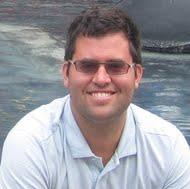
\includegraphics[height=1.25in]{mike.jpg}} & \\
  & \\
  & Michael Mulhearn \\
  & mulhearn@physics.ucdavis.edu \\
  & Physics 317 \\
  & \\
\end{tabular}
\vskip 0.5cm

\noindent
\begin{tabbing}
\hspace*{8em} \= \kill 
\textbf {Lecture:} \> Thursday 3:10-4:00 PM in Roessler 55 
\end{tabbing}
\noindent
\begin{tabbing}
\hspace*{8em} \= \kill 
\textbf{Textbooks:} \> Intro. to Quantum Mechanics (3rd Ed.) by Griffiths and Schroeder\\
\> ~~~(Recommended for reference, or any other Intro. QM text.)\\
\> Lecture notes on Scientific Python (link on course site)\\
\end{tabbing}
\noindent
\begin{tabbing}
\hspace*{8em}\= \hspace*{10em} \= \kill 
\textbf{Course TA:} \> TBD \> (TBD@ucdavis.edu)
\end{tabbing}
\noindent
\begin{tabbing}
\hspace*{8em}\= \hspace*{10em} \= \kill 
\textbf{Office Hours:}
    \> Mulhearn: \> TBD \\
    \> TBD: \> TBD
\end{tabbing}
\noindent
\begin{tabbing}
\hspace*{12em}\= \kill 
\textbf{Exams:} \> No Exams!\\
\textbf{Quizes:} \> Up to five in-class prove-you-wrote-it quizzes.\\
\textbf{Final Project:} \> Due March, 21 2024 10:30 AM \\
\end{tabbing}
\noindent
\textbf {Course Description:}\\
Applications of computational physics to problems from Classical and Quantum Mechanics.
You will bring the Schr\"odinger Equation to life!  Application of numerical techniques, and comparison to analytic solutions (where they exist).  Visualization of the wave function and its time evolution.  Applications of the Discrete Fourier transform.\\[8pt]
\noindent
\textbf {Course Philosophy:}\\
Computational physics is essential to nearly every career related to physics.  Unfortunately, the educational pipeline, since grade school, does not adequately prepare students with programming skills, and so a central feature of computational physics courses is a wide distribution of student programming abilities.  There are students that are better programmers than most physics professors, students that have little practice outside of the required computational courses, and everything in between.
Fortunately, in this course we are concerned with {\bf computational physics} and not just {\bf computer programming}.  You do not need to be an expert computer programmer to succeed in this course. You do need to gain enough programming competency to handle the fascinating physics problems we will tackle.  {\bf The primary objective of this course is to make you confident in using programming independently as an essential and effective tool for solving physics problems.}\\[3pt]

\noindent
This is a one unit course, and I will do my best to keep the workload appropriate.  However, given the wide variation in student programming abilities, inevitably some students will find the homework more time-consuming than others.  If you do find yourself working longer on the assignments, please understand that this is time well-spent:  gaining more proficiency in computing is almost certainly one of the best possible uses of your time at this stage in your career.\\[3pt]

\noindent
\textbf{Homework:}\\
There will be up to five home-work assignments which will feature problems in computational physics.
In general, you will have two weeks to complete each home-work, as will be detailed on the course website.  You may discuss the problems with other students, but you should write your own code, and make certain that you understand it, or else you will struggle with the homework quizzes.\\[3pt]

\noindent
\textbf{Quizes:}\\
In the lecture following each assignment, you will usually take a short quiz.  The quizzes will be intended to test that you understood the code you submitted to complete each assignment.  They will often feature Parson's problems:  programming puzzles that force you to specify the order in which provided lines of code should be arranged to answer a given prompt.\\[3pt]

\noindent
\noindent
\textbf{Final Project:}\\
In lieu of a final exam, you will design an independent creative problem.  While your particular problem may be solved online, your solution should vary substantially from anything available online.\\[3pt]

\noindent
\textbf {Grades:}\\
Final grades will be approximately $40\%$ Homework, $40\%$ Quizzes, and
$20\%$ Final Project.  Your worst quiz score will be dropped.  You will be allowed to submit one homework assignment late, but you must complete every assignment to complete the course.
You must also pass each component of the course (homework, quizzes, and final project) in order to pass the course.  The passing level may be adjusted (lower than $60\%$) at my discretion. As this is the first time this course has been taught, I may adjust the relative weighting of each contribution to your final score, based on my observation of typical student outcomes.\\
\noindent
\end{document}

